\begin{abcliste}
\abc
\begin{center}
\begin{tabular}{l|cccccc}
$t$ in \si{\second} & $0$ & $1$ & $2$ & $3$ & $4$ & $5$ \\
\hline
$s$ in \si{\meter} & $0$ & $0.5$ & $2$ & $4.5$ & $8$ & $12.5$ \\
\hline
$\Delta s$ in \si{\meter} & & $0.5$ & $1.5$ & $2.5$ & $3.5$ & $4.5$
\end{tabular}
\end{center}
Die Abstände zwischen den Punkten werden von Sekunde zu Sekunde grösser: Der Wagen wird immer schneller. Im $s(t)$-Diagramm wird der Graph deshalb immer steiler. Er beginnt waagrecht und ist eine $\result{\text{nach oben gekrümmte Kurve (Parabel)}}$ (blau):
\begin{center}
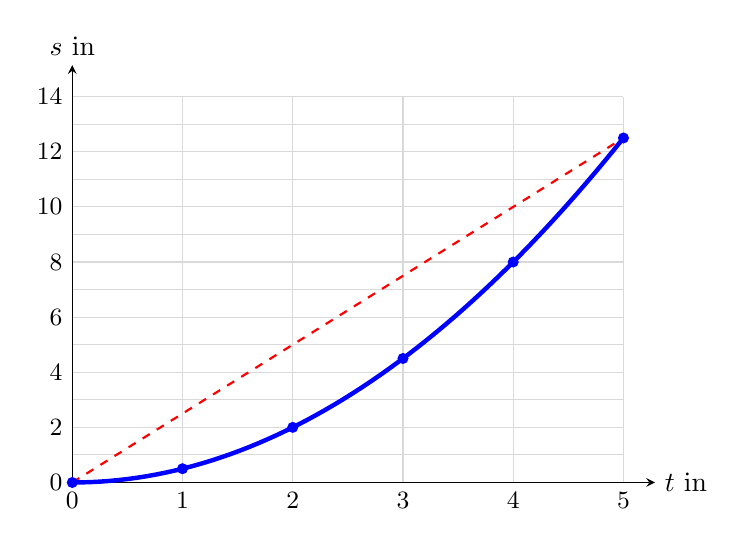
\begin{tikzpicture}[>=stealth, x=1.4cm, y=0.35cm]
 \draw[gray!30] (0,0) grid[xstep=1, ystep=1] (5,14);
 \draw[->] (0,0) -- (5.286,0) node[right] {$t$ in \si{\second}};
 \draw[->] (0,0) -- (0,15.143) node[above] {$s$ in \si{\meter}};
 \foreach \tk in {0,1,2,3,4,5} \node[below] at (\tk,0) {\small $\tk$};
 \foreach \yk in {0,2,4,6,8,10,12,14} \node[left] at (0,\yk) {\small $\yk$};

 \draw[thick, red, dashed] (0,0) -- (5,12.5);
 \draw[ultra thick, blue, domain=0:5, samples=60] plot (\x, {0.5*\x*\x});
 \fill[blue] (0,0) circle (2pt);
 \fill[blue] (1,0.5) circle (2pt);
 \fill[blue] (2,2) circle (2pt);
 \fill[blue] (3,4.5) circle (2pt);
 \fill[blue] (4,8) circle (2pt);
 \fill[blue] (5,12.5) circle (2pt);
\end{tikzpicture}
\end{center}
\abc Eine Gerade im $s(t)$-Diagramm hat überall dieselbe Steigung: Sie beschreibt eine gleichförmige Bewegung mit
\begin{align}
 v &= \vLineF = \frac{\sEnd}{\tEnd} = \vLine \approx \vLineP{0}{2}
\end{align}
(rot gestrichelt). Dann müssten die Punkte im Stroboskopbild gleiche Abstände von \SI{2.5}{\meter} haben. Das ist nicht der Fall: Der Wagen ist am Anfang langsamer und am Ende schneller als \vLineP{0}{2}. Die Gerade stimmt nur am Anfang und am Ende mit dem Ort überein; dazwischen liegt sie über den gemessenen Orten. $\result{\text{Die Gerade ist falsch}}$: \vLineP{0}{2} ist nur die mittlere Geschwindigkeit.

Die Punkte dürfen also nicht einfach mit dem ersten und dem letzten verbunden werden; jeder gemessene Ort muss im Diagramm erscheinen.
\end{abcliste}
